%%%%%%%%%
\section{Signal modeling}\label{sec:signalModel}
%%%%%%%%%

The potential discovery and exclusion power of these analyses rely on the ability of finding a local enhancement on the top of a smoothly falling background. 
This is ultimately achieved through an unbinned likelihood fit of the signal + background model to the reconstructed diboson invariant mass, which depends on the accurate description of the signal shape.

An analytical parametrization of the signal shape is chosen such that it well reproduces the simulated resonance distributions.
As stated in Section~\ref{subsec:signalMC}, simulated signal events are generated with a resonance natural width sufficiently small compared to the detector resolution.
This makes the model used for generating the events independent from the detector effects on the signal shape, allowing a model independent search for narrow resonances
where only the detector resolution has to be described. A double-sided Crystal-Ball (CB) function~\cite{CrystalBallRef} (i.e. a Gaussian core with power law tails on both sides) is found to well serve this purpose.
To take into account differences between muon and electron momentum resolutions, the signal invariant mass distribution is parametrized separately in the two lepton flavor categories.

Figure~\ref{fig:mWHfit-signal-8TeV} shows an example for the fitted signal distribution through a CB function for a \Wpr mass of 1.5\TeV in the muon channel of the $\ell\nu$+H-jet analysis.
Other examples are shown in Fig.~\ref{fig:mWVfit-signal-13TeV}, for the $\ell\nu$+V-jet analysis in the muon channel, for several signal hypotheses and for both \mJ categories.

\begin{figure}[!htb]
\centering
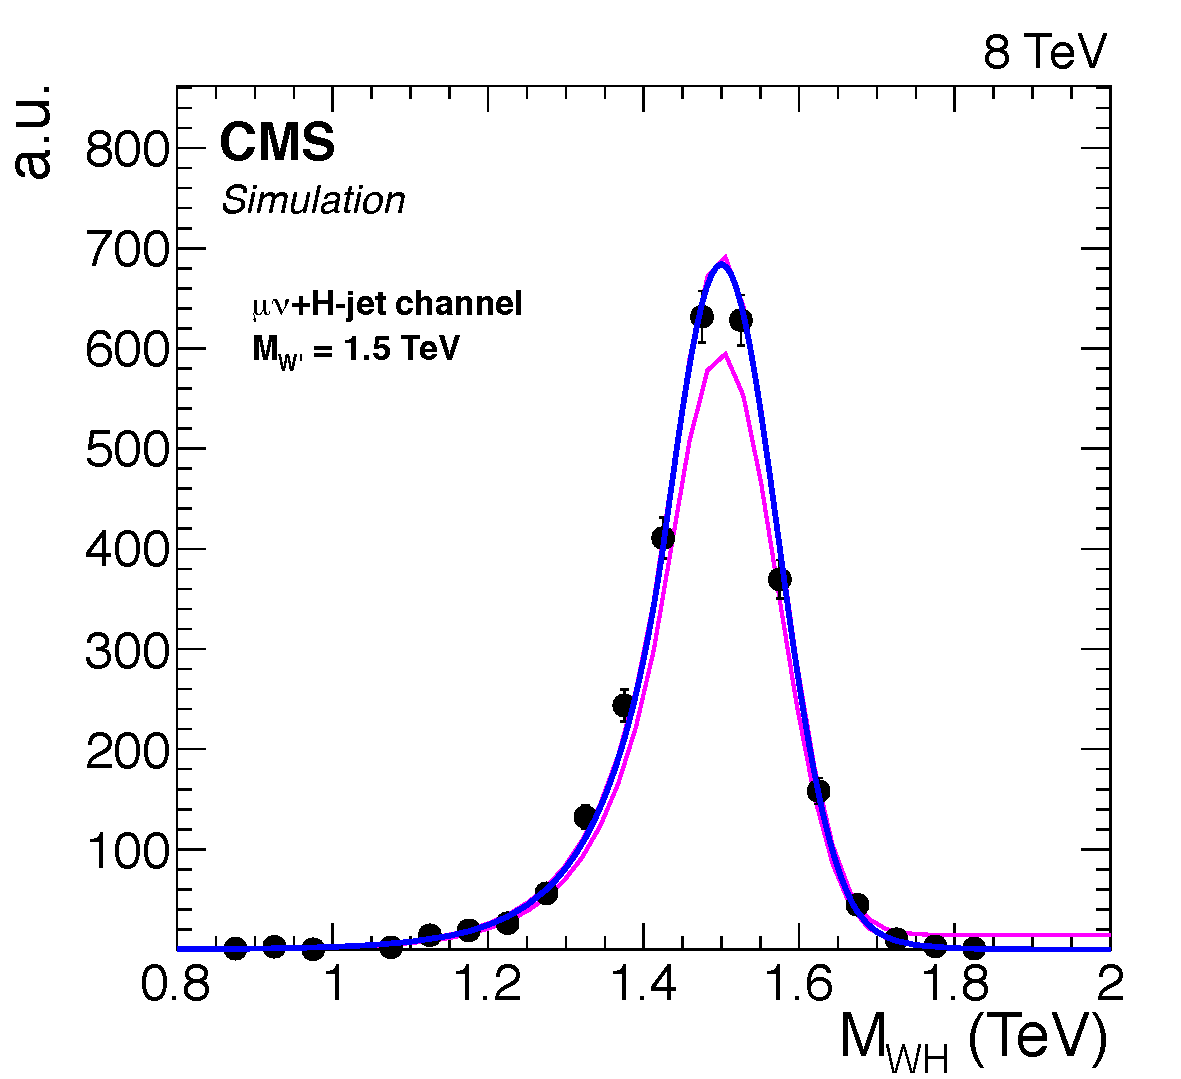
\includegraphics[width=0.5\textwidth]{\cheight/mWH-signal-mu-8TeV.pdf}
\caption{blabla}
\label{fig:mWHfit-signal-8TeV}
\end{figure}

\begin{figure}[!htb]
\centering
\subfigure[]{\label{fig:mWVfit-signal-13TeV_a}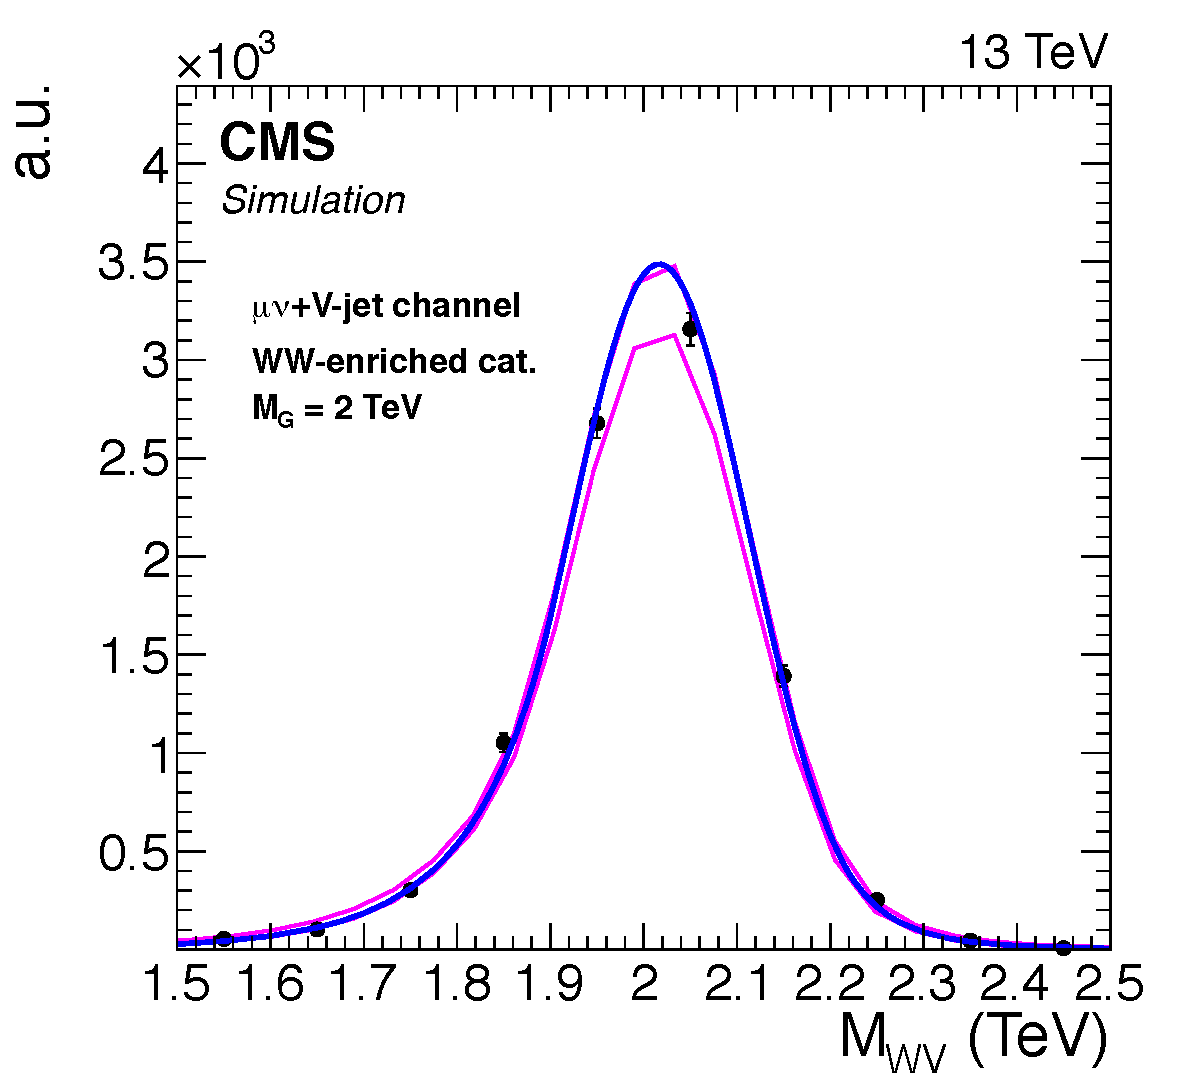
\includegraphics[width=0.3\textwidth]{\cheight/mWV-signal-bulkg-mu-HPW-13TeV.pdf}}
\subfigure[]{\label{fig:mWVfit-signal-13TeV_b}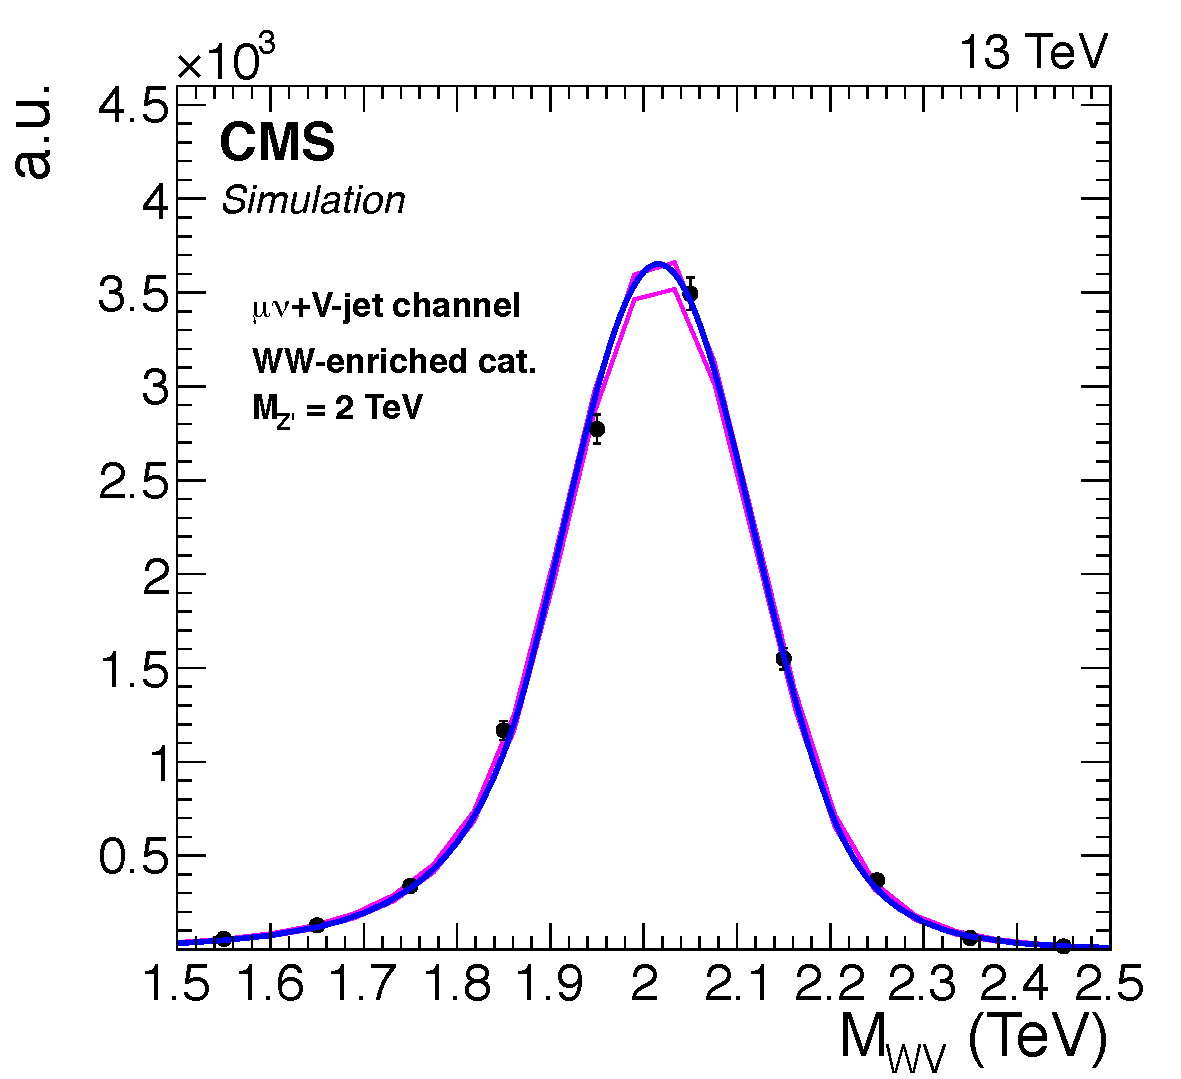
\includegraphics[width=0.3\textwidth]{\cheight/mWV-signal-zprime-mu-HPW-13TeV.pdf}}
\subfigure[]{\label{fig:mWVfit-signal-13TeV_c}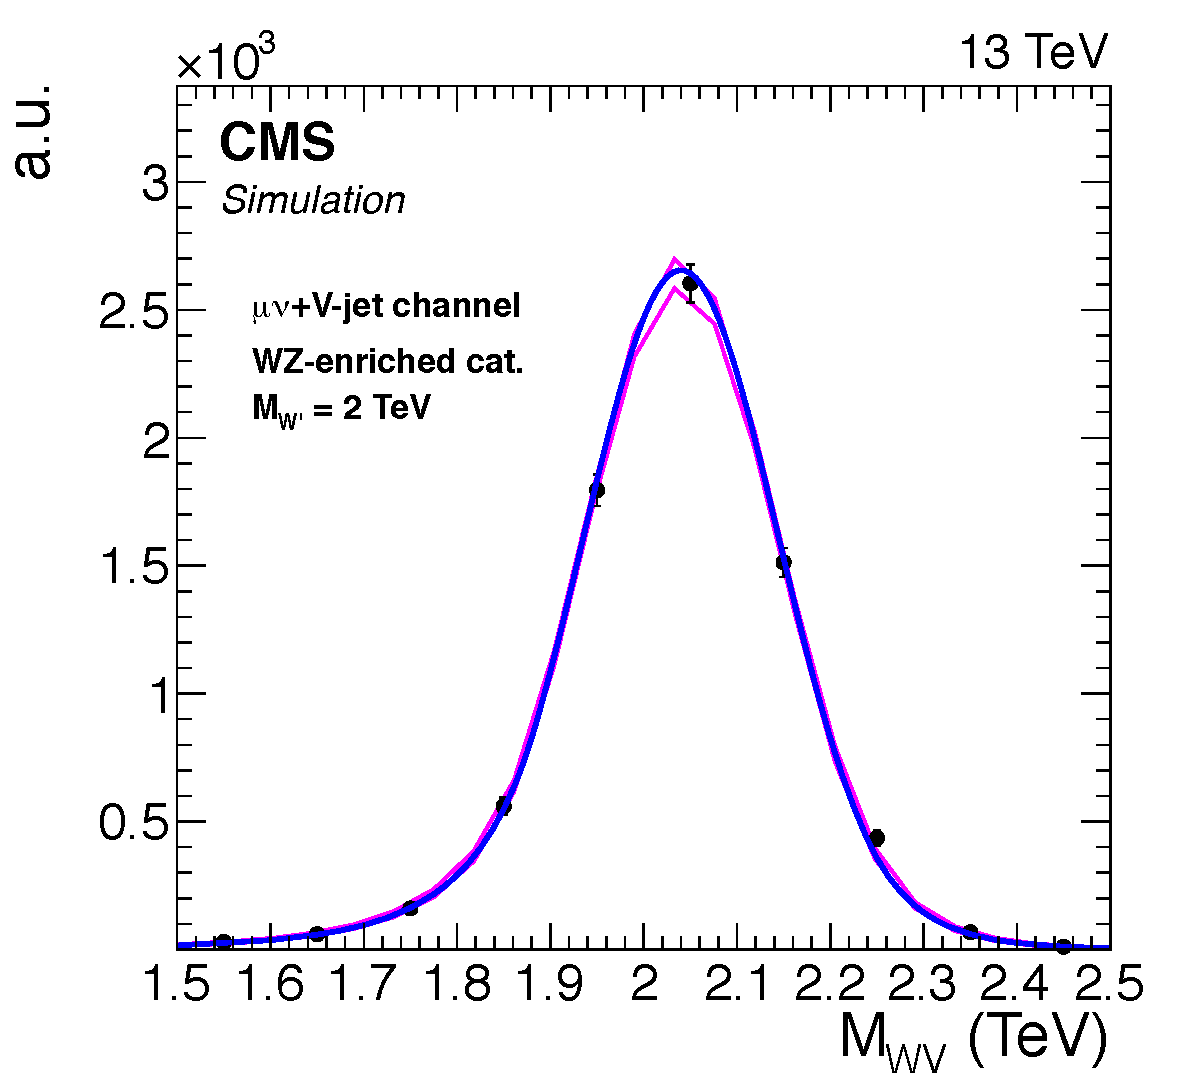
\includegraphics[width=0.3\textwidth]{\cheight/mWV-signal-wprime-mu-HPZ-13TeV.pdf}}
\caption{blabla}
\label{fig:mWVfit-signal-13TeV}
\end{figure}

Because of the limited number of available simulated samples, a liner interpolation is performed for each parameter of the CB function between
the shapes obtained for some reference mass points, in order to extrapolate the distribution for intermediate values of the resonance mass.
The resolution of the reconstructed diboson invariant mass is given by the width of the Gaussian core and it ranges between 7 and 4\% depending on the resonance mass, as shown in Fig.~\ref{fig:relCB}.
The resolution is dominated by the jet and \ETmiss contibutions.

\begin{figure}[!htb]
\centering
\subfigure[]{\label{fig:relCB_a}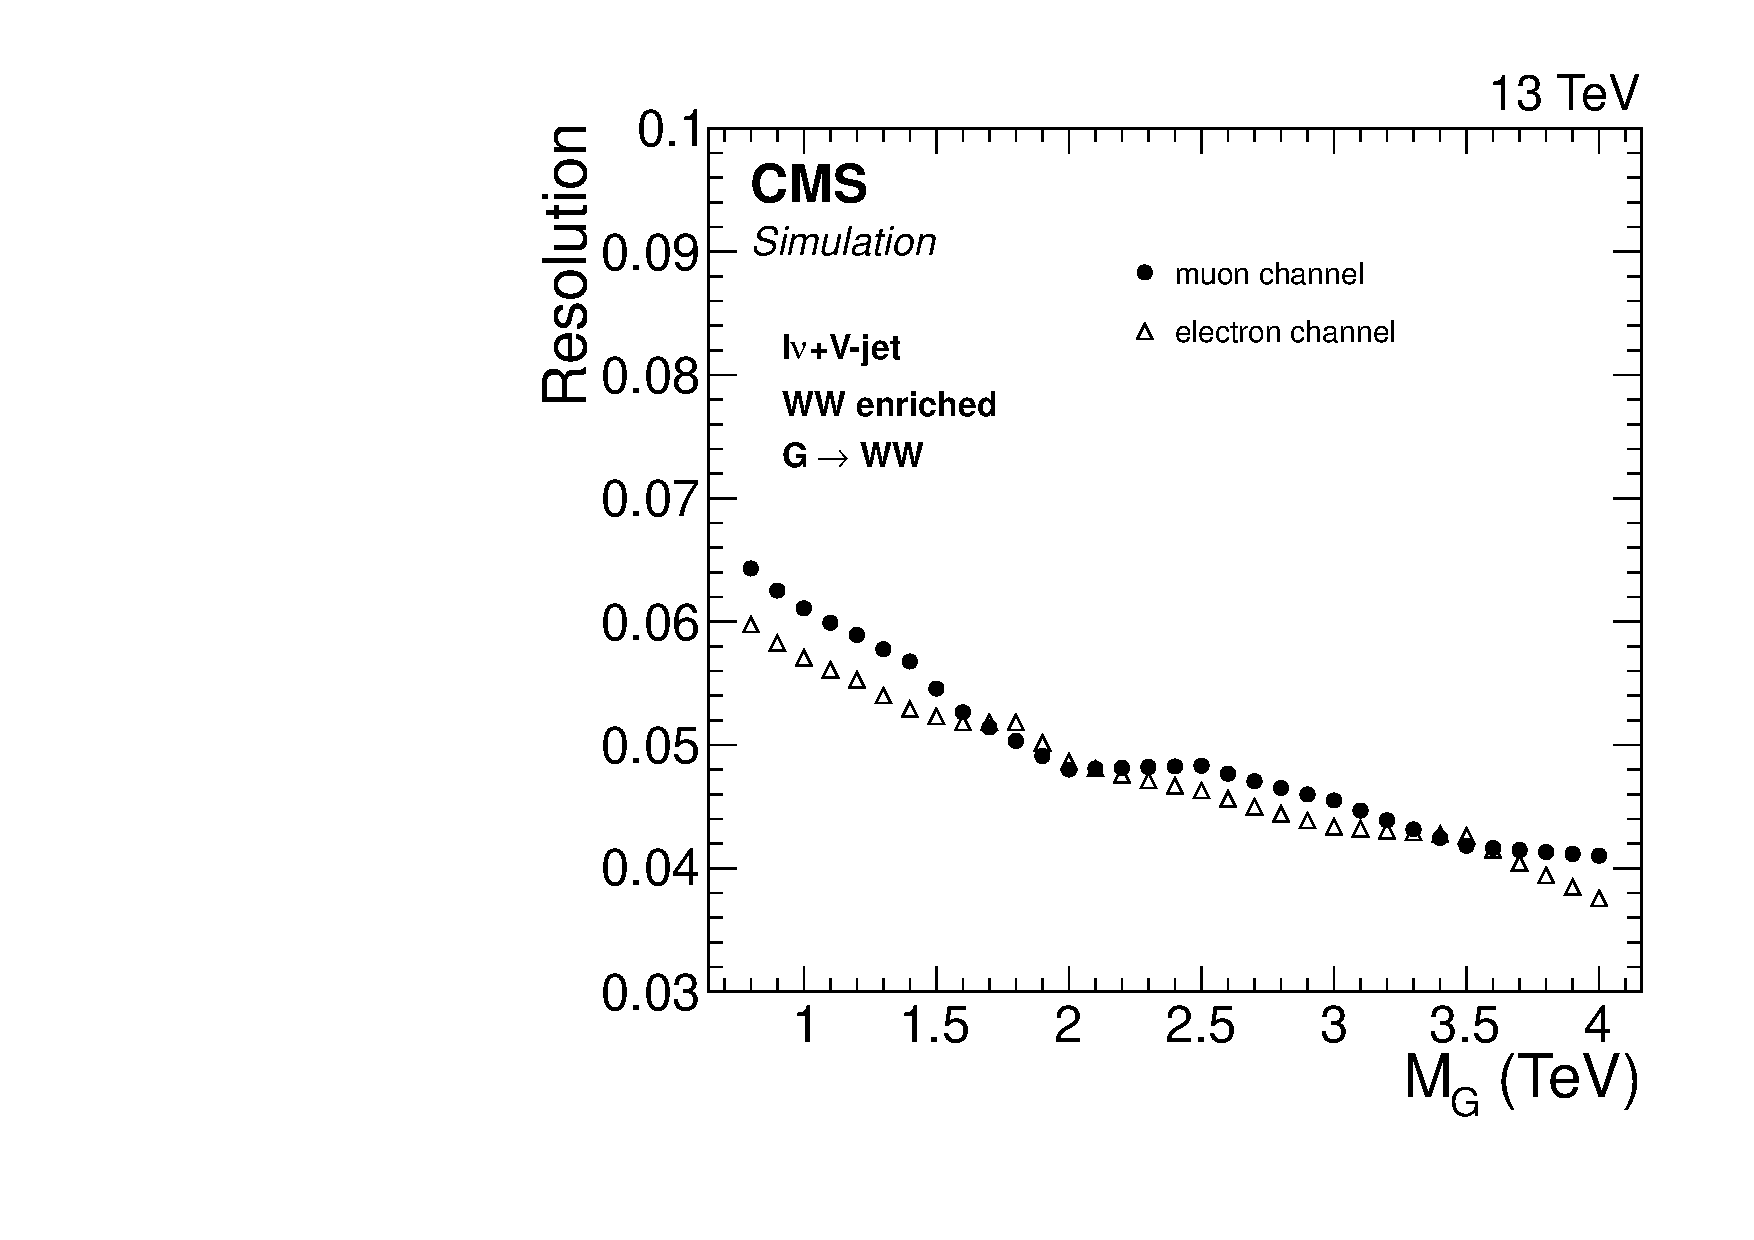
\includegraphics[width=0.3\textwidth]{\cheight/CBrel-bulkg-HPW-13TeV.pdf}}
\subfigure[]{\label{fig:relCB_b}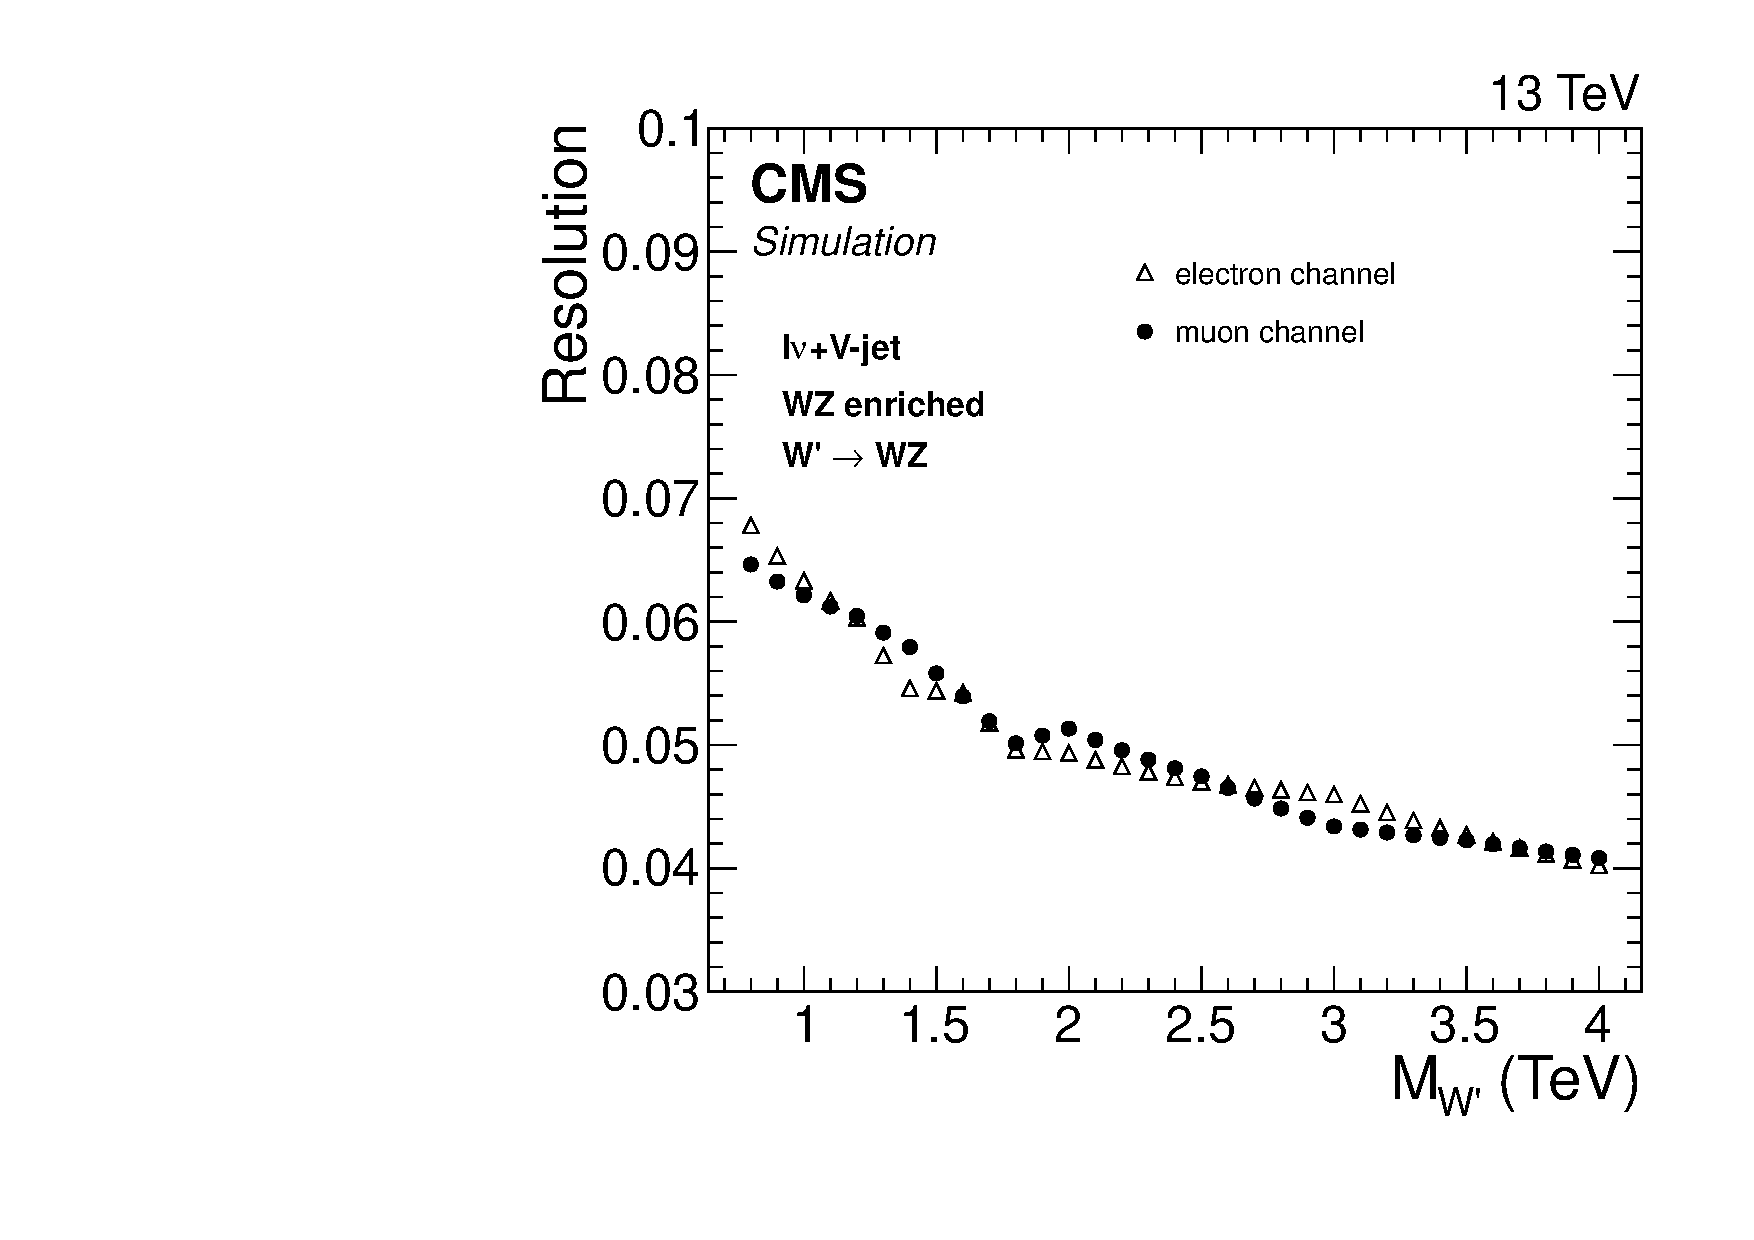
\includegraphics[width=0.3\textwidth]{\cheight/CBrel-wprime-HPZ-13TeV.pdf}}
\subfigure[]{\label{fig:relCB_c}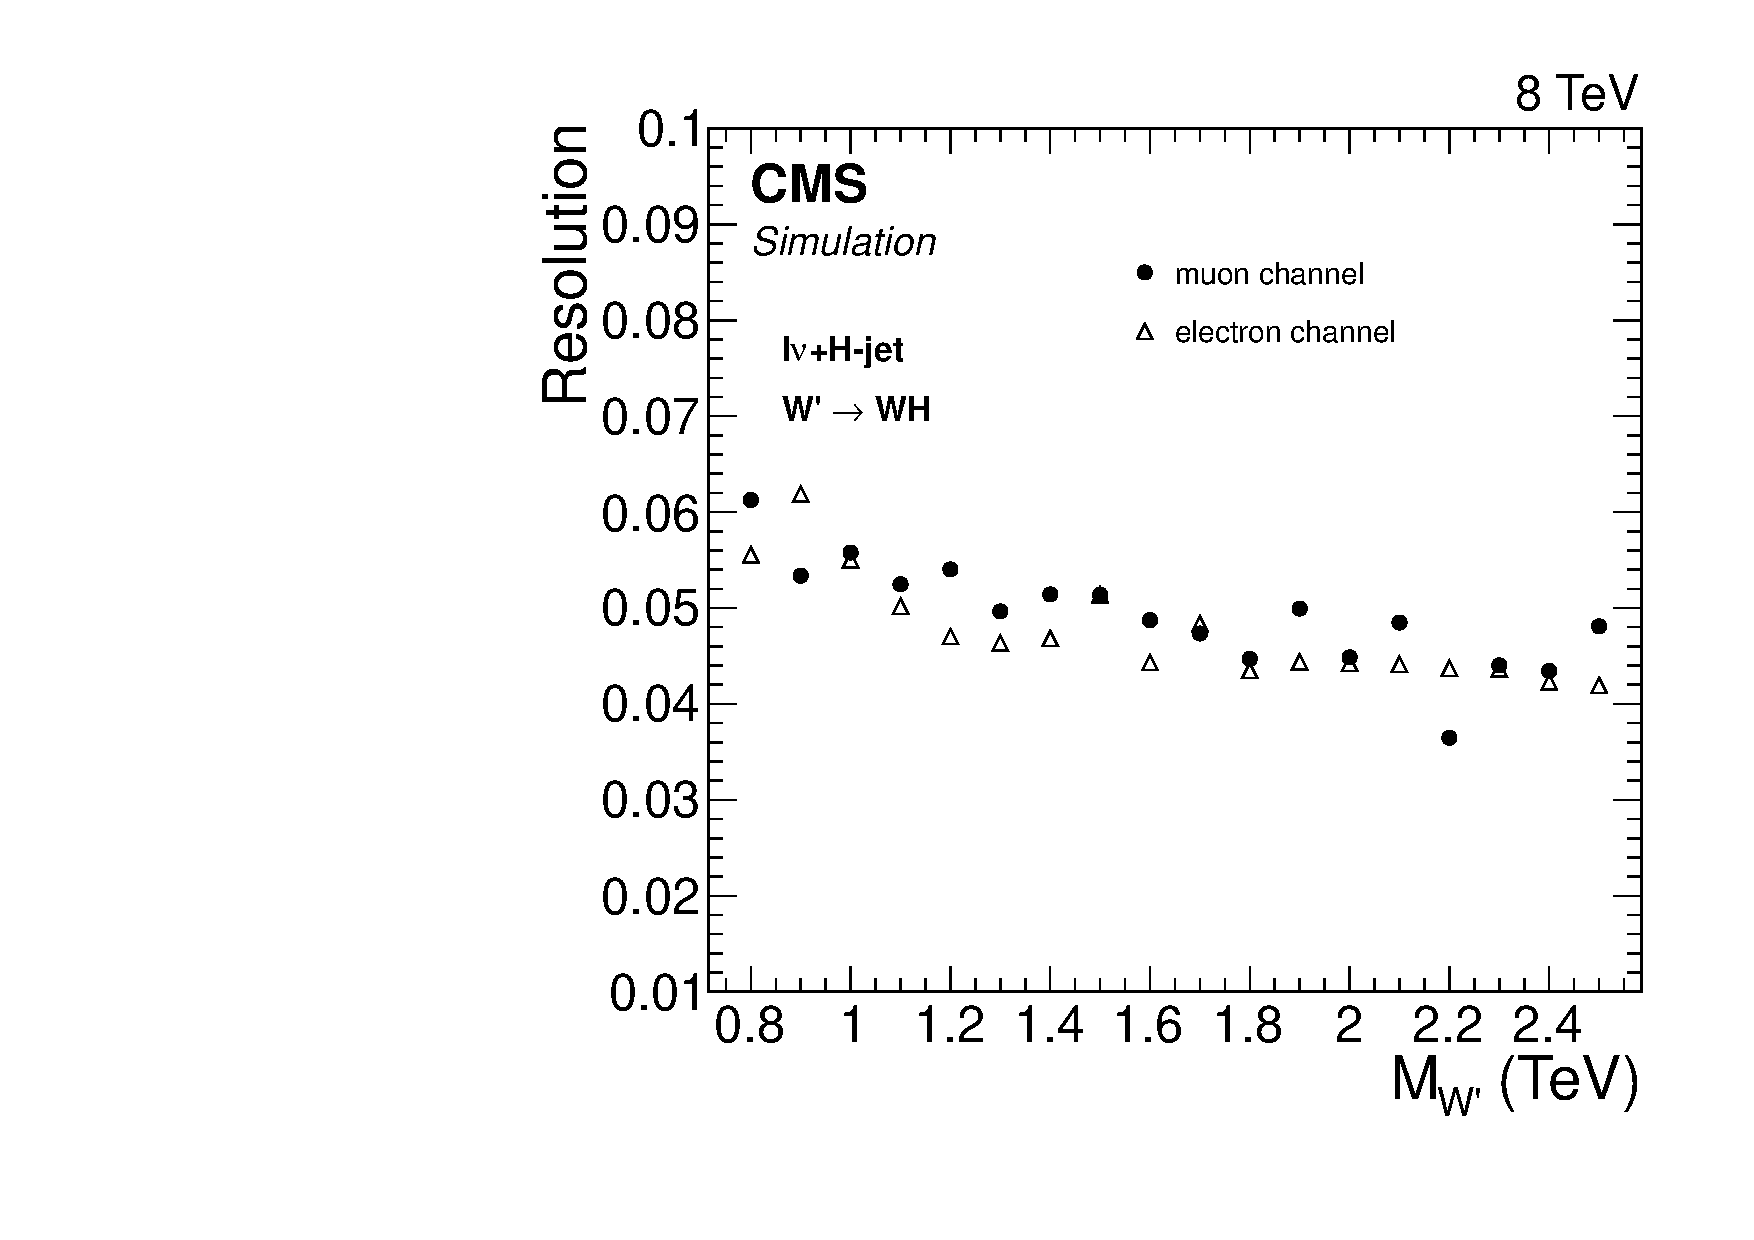
\includegraphics[width=0.3\textwidth]{\cheight/CBrel-wprime-WH-8TeV.pdf}}
\caption{blabla}
\label{fig:relCB}
\end{figure}

The signal selection efficiency, evaluated for each category, is defined as the number of selected signal events over the number of generated ones, which include all the possible lepton flavours (e, $\mu$ and $\tau$).
As shown in Figure~\ref{fig:effWV-13TeV} the efficiency for a $\Zpr$ or bulk graviton signal in the WW-enriched category is $\approx$ 2 times larger compared to a $\Wpr$ signal. On the other hand, the efficiency for a $\Wpr$ signal in the WZ-enriched category is $\approx$ 4 times larger compared to a $\Zpr$ or bulk graviton signal. For both categories and for each signal hypothesis the efficiency is smaller compared to the large \mJ window used for V tagging. However, the resulting loss in sensitivity in each of the category is recovered with a combination of the two \mJ categories which allows the use of all the available data. With this solution the discrimination between the two type of signals is maximized together with a gain in sensitivity of 10--20\% depending on the resonance mass.

A linear interpolation of the signal efficiency is performed between the values obtained for some reference mass points in order to extrapolate the efficiency for intermediate resonance masses for which a simulated sample is not available.
The efficiency for the electron channel is lower compared to the muon channel over most of the phase space due to the tighter requirements on the electron \pt and \ETmiss. This effect is less visible in the $\ell\Pgn$+H-jet channel (see Fig.~\ref{fig:effWH-8TeV}) where the electron selections are less strict. For all cases, at low masses the efficiency increases with the resonance mass because of the increase in the acceptance of the lepton, \ETmiss and $m_\mathrm{WV/WH}$ selections together with the inefficiency of the jet algorithms in reconstructing the merged jet for a low boosted V boson (\FIXME{point to figure}). At larger resonance masses the efficiency slightly decrease due to \nsubj selection inefficiency for high \pt V jets, as described in Section~\ref{sec:vtagging}.
For the electron channel this effect is compensated by a larger increase in the lepton selection acceptance, resulting in a nearly flat efficiency at high resonance masses.
Similar considerations hold for the efficiency in the $\ell\Pgn$+H-jet channel shown in Fig.~\ref{fig:effWH-8TeV}.

\begin{figure}[!htb]
\centering
\subfigure[]{\label{fig:effWV-13TeV_a}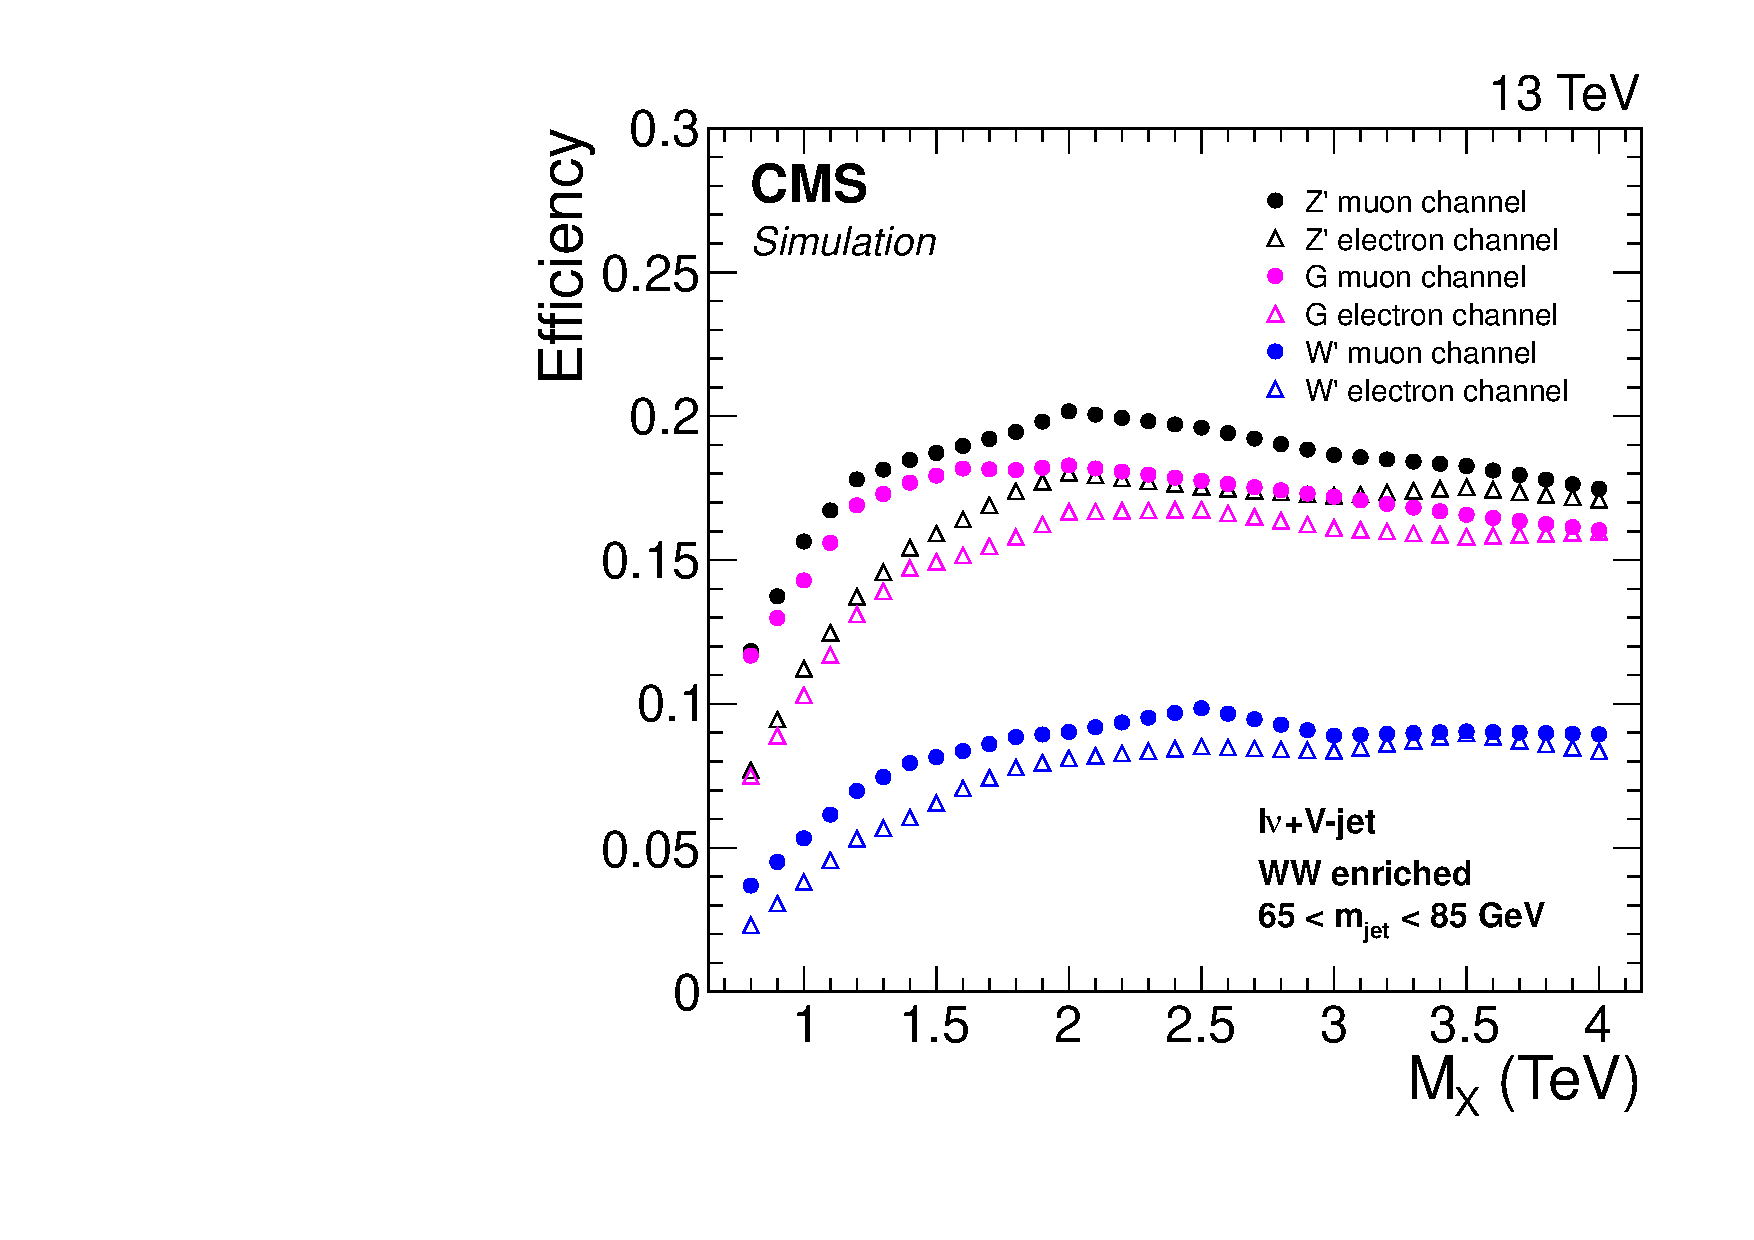
\includegraphics[width=0.3\textwidth]{\cheight/signal-eff-HPW-all.pdf}}
\subfigure[]{\label{fig:effWV-13TeV_b}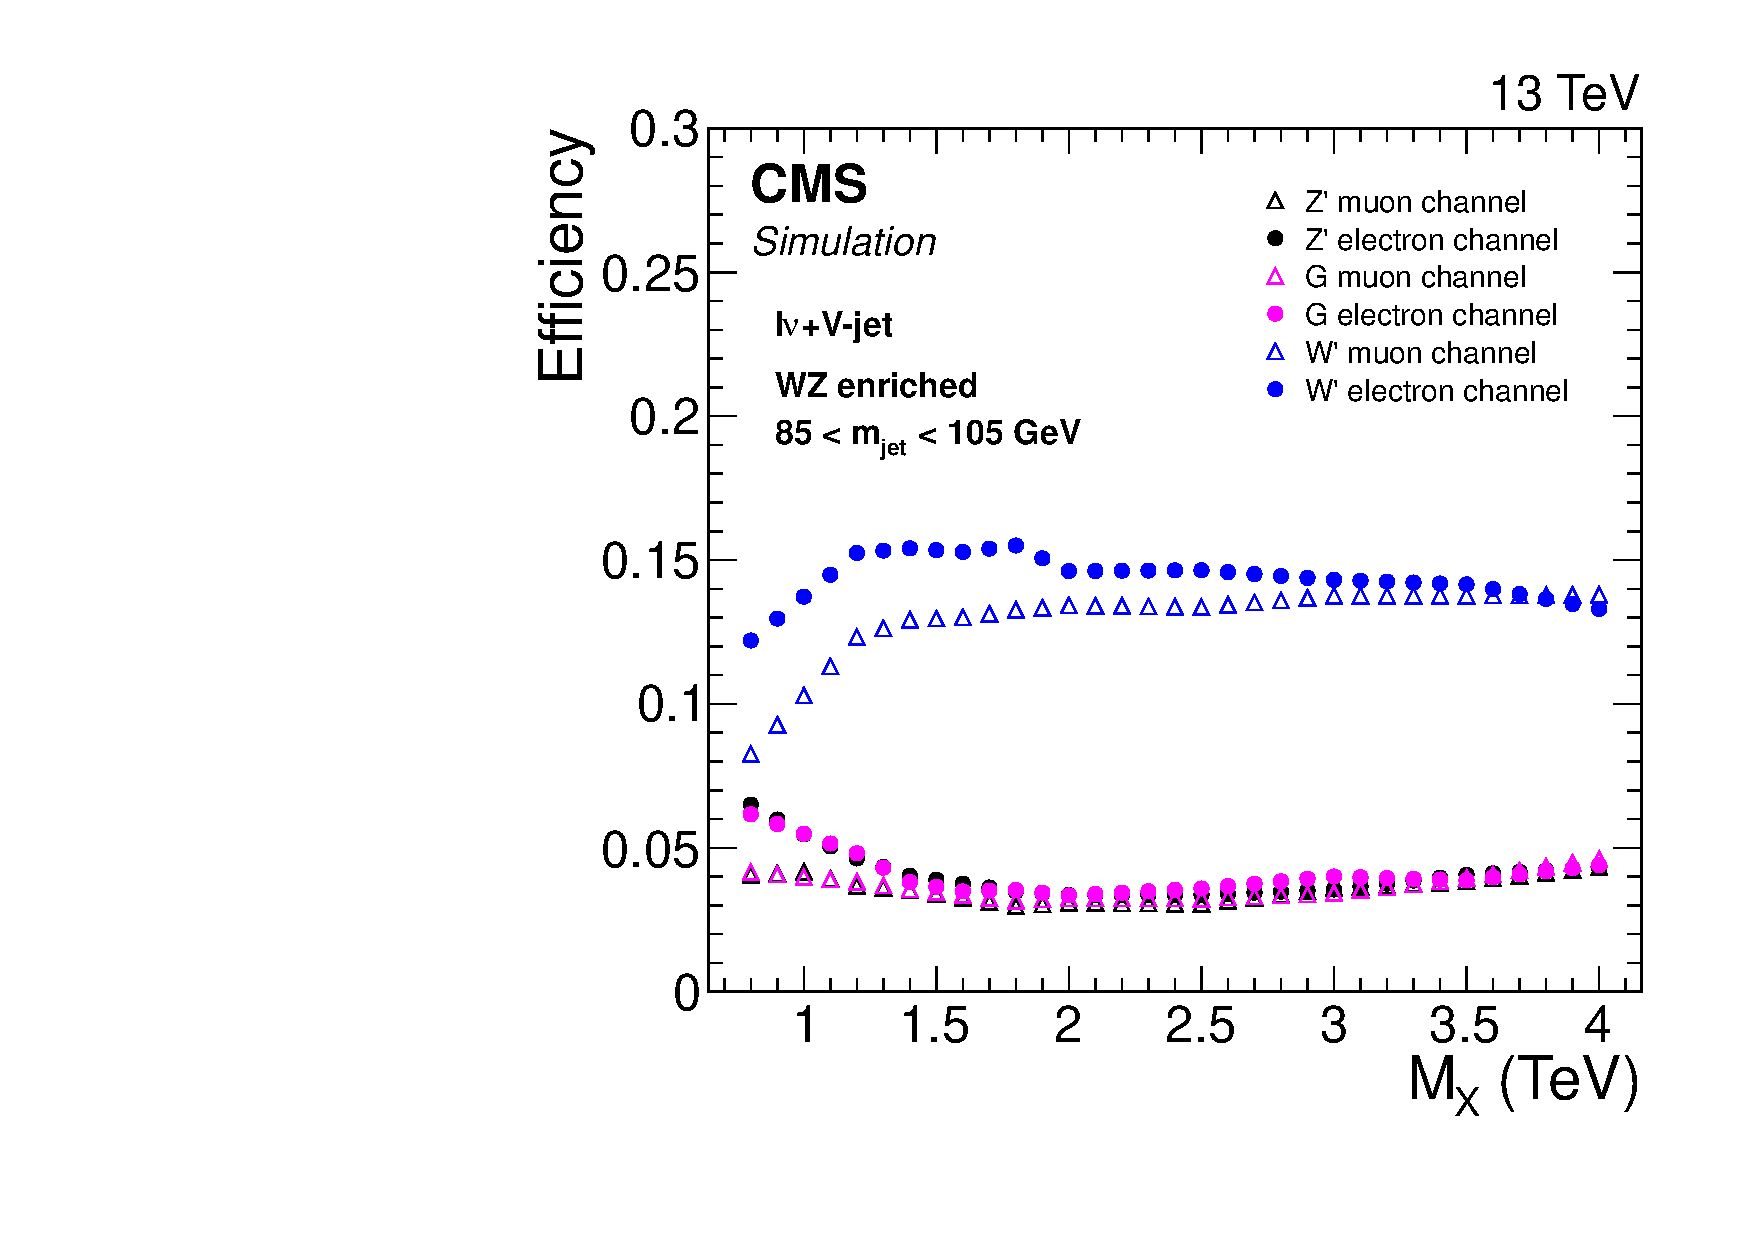
\includegraphics[width=0.3\textwidth]{\cheight/signal-eff-HPZ-all.pdf}}
\subfigure[]{\label{fig:effWV-13TeV_c}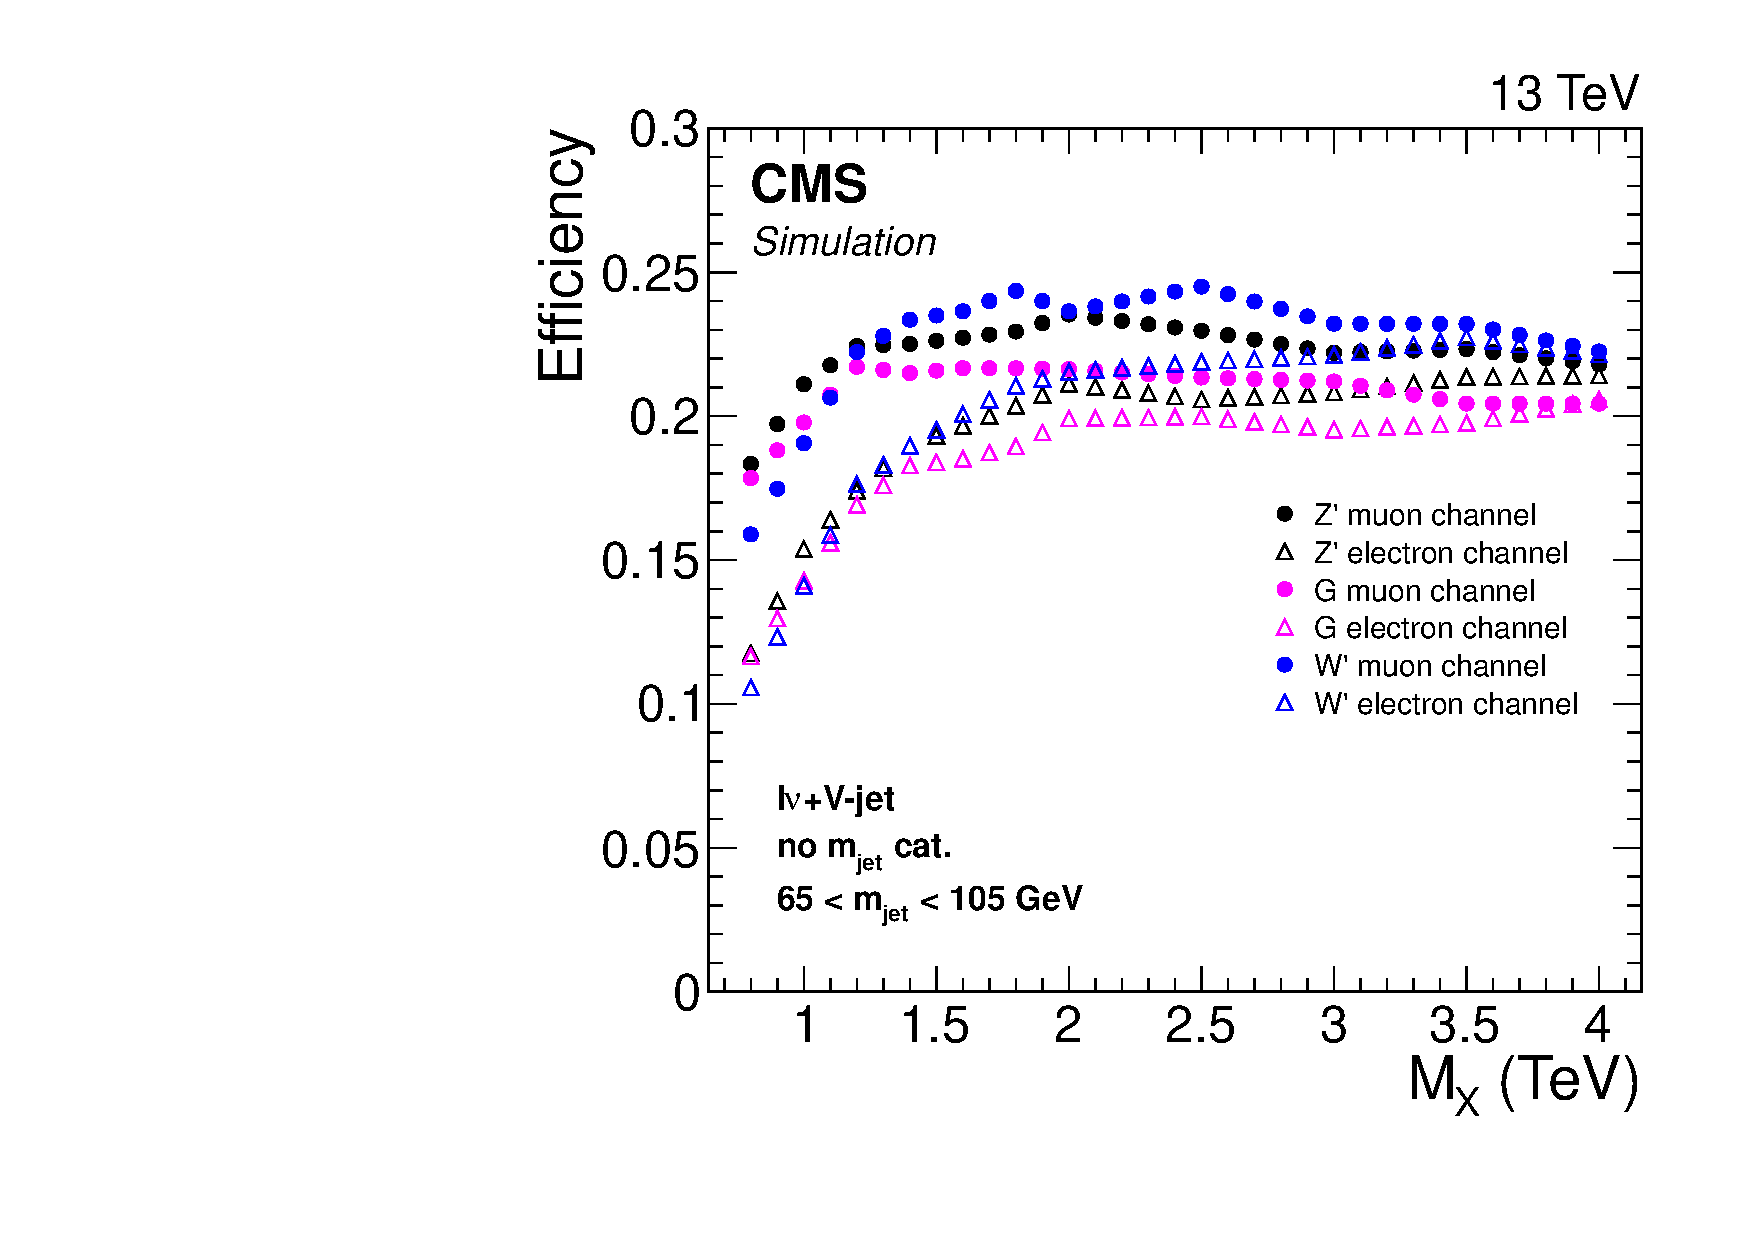
\includegraphics[width=0.3\textwidth]{\cheight/signal-eff-HP-all.pdf}}
\caption{blabla}
\label{fig:effWV-13TeV}
\end{figure}

\begin{figure}[!htb]
\centering
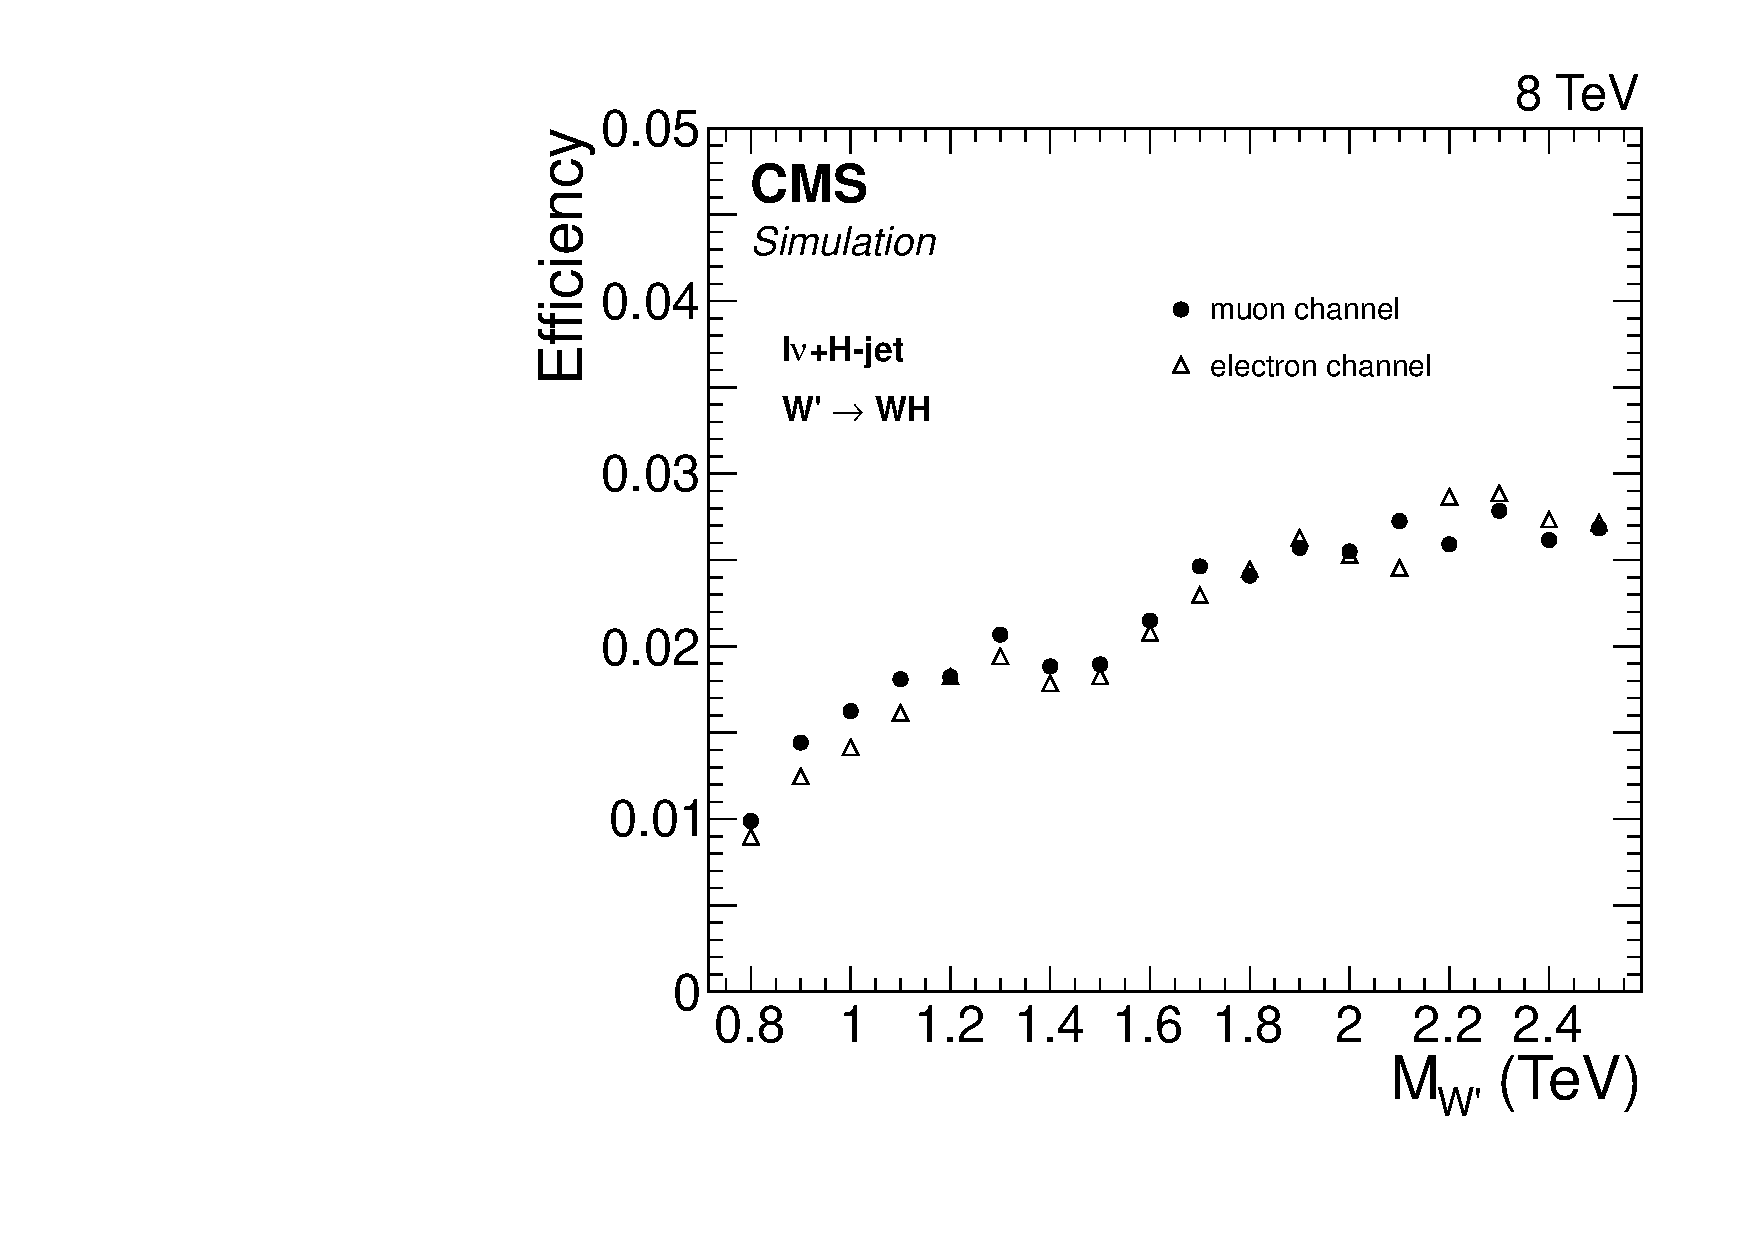
\includegraphics[width=0.5\textwidth]{\cheight/signal-eff-WH.pdf}
\caption{blabla}
\label{fig:effWH-8TeV}
\end{figure}